\documentclass[10pt,conference,compsocconf]{IEEEtran}
\usepackage{graphicx}
\usepackage{booktabs}
\usepackage{amsmath}
\usepackage[hidelinks]{hyperref}

\begin{document}
\title{Predicting Coronary Heart Disease from the BRFSS Survey\\with NumPy Gradient Boosting and Embedding Networks}
\author{\IEEEauthorblockN{Ruhan Liu, Yun-Chia Shih, Jingru Wang}
\IEEEauthorblockA{EPFL, Machine Learning course, Fall 2026}}
\maketitle

\begin{abstract}
We predict self-reported myocardial infarction or coronary heart disease (MICHD) for
109,379 respondents of the 2015 BRFSS telephone survey, scored by F1 on the positive class.
Using only NumPy, we implement a histogram gradient-boosted decision tree (GBDT) and an
entity-embedding neural network, train them on all labelled rows and blend their log-odds.
Under 5-fold cross-validation the ensemble reaches F1 0.4487 (average precision
0.4380), against 0.4290 for the best linear baseline built from the required methods;
on the AIcrowd test set it scores \textbf{F1 0.460} (accuracy 0.881), our best submission. We show that the remaining error is dominated by overlap between classes, that
leaderboard noise ($\pm0.003$) is as large as most model changes, and that more training
data still helps.
\end{abstract}

\section{Introduction}
The data contain 328,135 labelled and 109,379 unlabelled respondents with 321 survey fields
(answers coded as in the CDC codebook, many missing by design). Only 8.83\% of labels are
positive, so predicting ``no disease'' for everyone gives 91\% accuracy and F1 = 0. Our
goal is a well-ranked probability score plus a single decision threshold that maximises
F1. All code uses NumPy and the Python standard library only.

\section{Methods}
\subsection{Evaluation protocol}
All numbers are out-of-fold (OOF) scores from 5-fold cross-validation stratified by label
(seed 2026), on all 328,135 rows with the natural class ratio. We report the best-threshold
F1 and the average precision (AP), a threshold-free summary of ranking quality that is less
noisy than F1. Every preprocessing statistic (bin edges, medians, scaling) is fitted on the
training folds only. To judge which differences matter we bootstrapped the OOF predictions
over random test-sized samples: test-set F1 has a standard deviation of \textbf{0.0034},
so differences below about 0.002 are not distinguishable on the leaderboard.

\subsection{Required methods and linear baselines}
\texttt{implementations.py} contains the six required methods (least squares via the normal
equations, ridge regression, MSE gradient descent and SGD with batch size 1, logistic and
$L_2$-regularised logistic regression by gradient descent). We use them as baselines on the
engineered features: training-fold 1st/99th-percentile clipping, median imputation,
standardisation and one missing-value indicator per incomplete column (448 inputs).

\subsection{Features}
(i) \emph{Codebook cleaning}: for 240 fields, ``don't know/refused'' codes (7/9, 77/99,
\dots) become $-1$, kept apart from ``not asked'' (missing), and ``none'' codes (88) become
0, so that ordinal splits are meaningful. (ii) Fourteen sampling-design and interview-date
fields are removed. (iii) Derived features: \emph{exact age}, recovered from the
pre-computed \texttt{MAXVO2\_} field, which is a linear function of un-capped age and sex
(\texttt{\_AGE80} is capped at 80); alcohol days per month; counts of chronic conditions,
activity limitations, unknown answers and missing answers. No column is dropped for
missingness: questionnaire routing is informative (e.g.\ all 773 respondents who answered
the cardiac-rehabilitation question \texttt{HAREHAB1} are positive).

\subsection{Binning}
Each of the 314 features is mapped to at most 64 integer bins: one bin per distinct value
when there are $\le 63$ values, otherwise 63 training quantiles; bin 0 is reserved for
missing. Both models below work on these bins.

\subsection{Gradient-boosted trees (GBDT)}
We implemented a histogram GBDT for the logistic loss. For each node the gradient and
Hessian sums per (feature, bin) are accumulated with \texttt{np.bincount}; the sibling of
the smaller child is obtained by histogram subtraction. Trees grow leaf-wise up to 31
leaves; a split maximises $G_L^2/(H_L+\lambda)+G_R^2/(H_R+\lambda)-G^2/(H+\lambda)$ over
thresholds and over sending the missing bin left or right, with $\ge$100--150 rows per
child. Leaves take Newton values $-G/(H+\lambda)$, $\lambda=5$. Two configurations are used:
\textbf{gbA} (600 trees, rate 0.03, 80\% row bagging, 50\% features per tree) and
\textbf{gbB} (1000 trees, rate 0.02, gradient-based one-side sampling keeping the 20\%
largest $|g|$ plus a reweighted 10\% of the rest, 40\% features, positive weight 2).

\subsection{Embedding neural network (NN)}
Every (feature, bin) pair has a learned 6-dimensional embedding; the 1,884 concatenated
values feed a 256--64 ReLU MLP with dropout 0.25. We train with Adam (rate $2\cdot10^{-3}$,
cosine decay, batch 1024, 4 epochs, $L_2=10^{-4}$ on embeddings), all gradients written by
hand. Positives get weight 4. Five random seeds are averaged.

\subsection{Ensemble and decision threshold}
Class weight $w$ multiplies the predicted odds by $w$, so each member's log-odds is
corrected by $-\log w$. The final score is $0.6\cdot$mean(gbA, gbB) $+\,0.4\cdot$mean(NN
seeds); any weight in 0.5--0.7 gives the same OOF F1 ($\pm0.0003$). The threshold is the
median of the F1-optimal thresholds on 50 bootstrap resamples of the OOF scores. For the
submission every member is retrained on \emph{all} labelled rows with 15\% more trees.

\section{Results}
\begin{table}[t]
\centering\caption{5-fold OOF results (328,135 rows). Rows in the lower blocks are ablations
of the configuration directly above them.}\label{tab:res}
\footnotesize\setlength{\tabcolsep}{4pt}
\begin{tabular}{lcc}
\toprule
Model & F1 & AP\\
\midrule
Ridge regression & 0.4290 & 0.4119\\
Reg.\ logistic reg.\ (300 GD steps) & 0.3114 & 0.2693\\
Logistic reg., 1/4 of negatives & 0.4224 & 0.3907\\
\midrule
gbB, raw columns (no feat.\ eng.) & 0.4477 & 0.4336\\
gbB (engineered features) & 0.4481 & 0.4352\\
gbA, 300 / 600 trees & 0.4464 / 0.4474 & 0.4346 / 0.4360\\
gbA with 63 leaves, $\lambda=20$ & 0.4450 & 0.4313\\
\midrule
NN, no class weight & 0.4435 & 0.4268\\
\quad + stronger regularisation & 0.4438 & 0.4290\\
\quad + positive weight 4 & 0.4462 & 0.4324\\
\quad + 5-seed average & 0.4471 & 0.4339\\
\midrule
\textbf{Blend (final)} & \textbf{0.4487} & \textbf{0.4380}\\
\bottomrule
\end{tabular}
\end{table}

Table~\ref{tab:res} summarises the experiments. The linear baselines built from the
required implementations (standardised features with median imputation and missingness
indicators; $\lambda=10^{-4}$ for ridge, $10^{-5}$ and step 0.5 for logistic) are clearly
weaker than both nonlinear models. Plain logistic GD converges slowly with a 9\% prior;
subsampling the negatives (equivalent to weighting positives $\times4$) fixes this but
still trails ridge. Interactions between age,
sex, general health and comorbidities matter. Feature engineering helps the trees by
+0.0016 AP. For the network, weighting the rare positive class improves the ranking
itself (+0.0034 AP), not only the threshold. The trees and the networks make different
errors, so blending adds +0.002 AP over the best single model.

\textbf{Rejected ideas} (no OOF gain): a third GBDT configuration (0.4485), ordinal bin
inputs to the NN (0.4446), randomly hiding 10\% of answers during NN training (0.4455),
and self-training on the test rows with soft pseudo-labels from the fold ensemble: the
student matched the teacher but added nothing to the blend ($<$0.0003 F1), because it
only distils information the ensemble already has.

\begin{figure}[t]
\centering
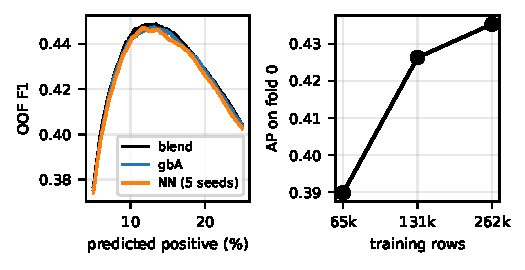
\includegraphics[width=\columnwidth]{report_fig.pdf}
\caption{Left: OOF F1 against the fraction of respondents predicted positive; the optimum
is flat between 11\% and 14\%. Right: learning curve of gbB on fold 0 (AP on the same
validation rows versus training rows, fixed hyper-parameters).}\label{fig:curves}
\end{figure}

\textbf{Threshold.} Figure~\ref{fig:curves} (left) shows that F1 is flat near its optimum,
so the exact threshold matters less than ranking quality; the chosen threshold predicts
13.2\% positives on OOF data and 13.3\% on the test set, confirming that the calibration
of the full-data models transfers.

\textbf{Bottleneck.} The learning curve (Fig.~\ref{fig:curves}, right) still rises by
+0.009 AP per doubling of the data, which is why the final models use all rows rather
than averaging 80\% fold models. Otherwise the problem is limited by information: positives
reported for respondents with few recorded risk factors are indistinguishable from
negatives: at the chosen threshold the OOF precision is 0.374 and recall 0.561
(accuracy 0.878).

\section{Discussion and conclusion}
The previous versions of our system (logistic baselines, then increasingly complex
calibrated tree and network stacks with subgroup thresholds) reached leaderboard F1
0.432--0.454 but local improvements smaller than the leaderboard noise. Replacing them by
two well-implemented model families, keeping all information (including missingness) and
training on all rows improves OOF AP by about 0.005 over the best previous component.
On AIcrowd this version (v7) scores \textbf{F1 0.460, accuracy 0.881}, our best result;
earlier versions scored 0.432 (logistic baseline), 0.436, 0.454, 0.444, 0.452 and 0.452.
The leaderboard F1 is 0.011 above the OOF estimate, in line with earlier versions
($\approx$0.008), the $\pm0.003$ test noise and the gain from full-data training.
Limitations: some signal comes from questionnaire routing (e.g.\ \texttt{HAREHAB1} is
asked only after a heart attack), so the model is a screening tool for this survey, not a
prospective clinical risk model; the label is self-reported; and CV hyper-parameter choices
reuse the same folds. Reproduction: \texttt{python run.py} regenerates the submission from
the saved models, \texttt{--train} retrains them (about 30 min) and \texttt{--cv}
recomputes all OOF predictions; \texttt{baselines.py} reproduces the linear baselines.

\end{document}
